\section{Appendix}



\begin{figure}[h]
  \centering
  \captionsetup[subfigure]{labelformat=empty}
  \begin{subfigure}[b]{1.0\textwidth}
    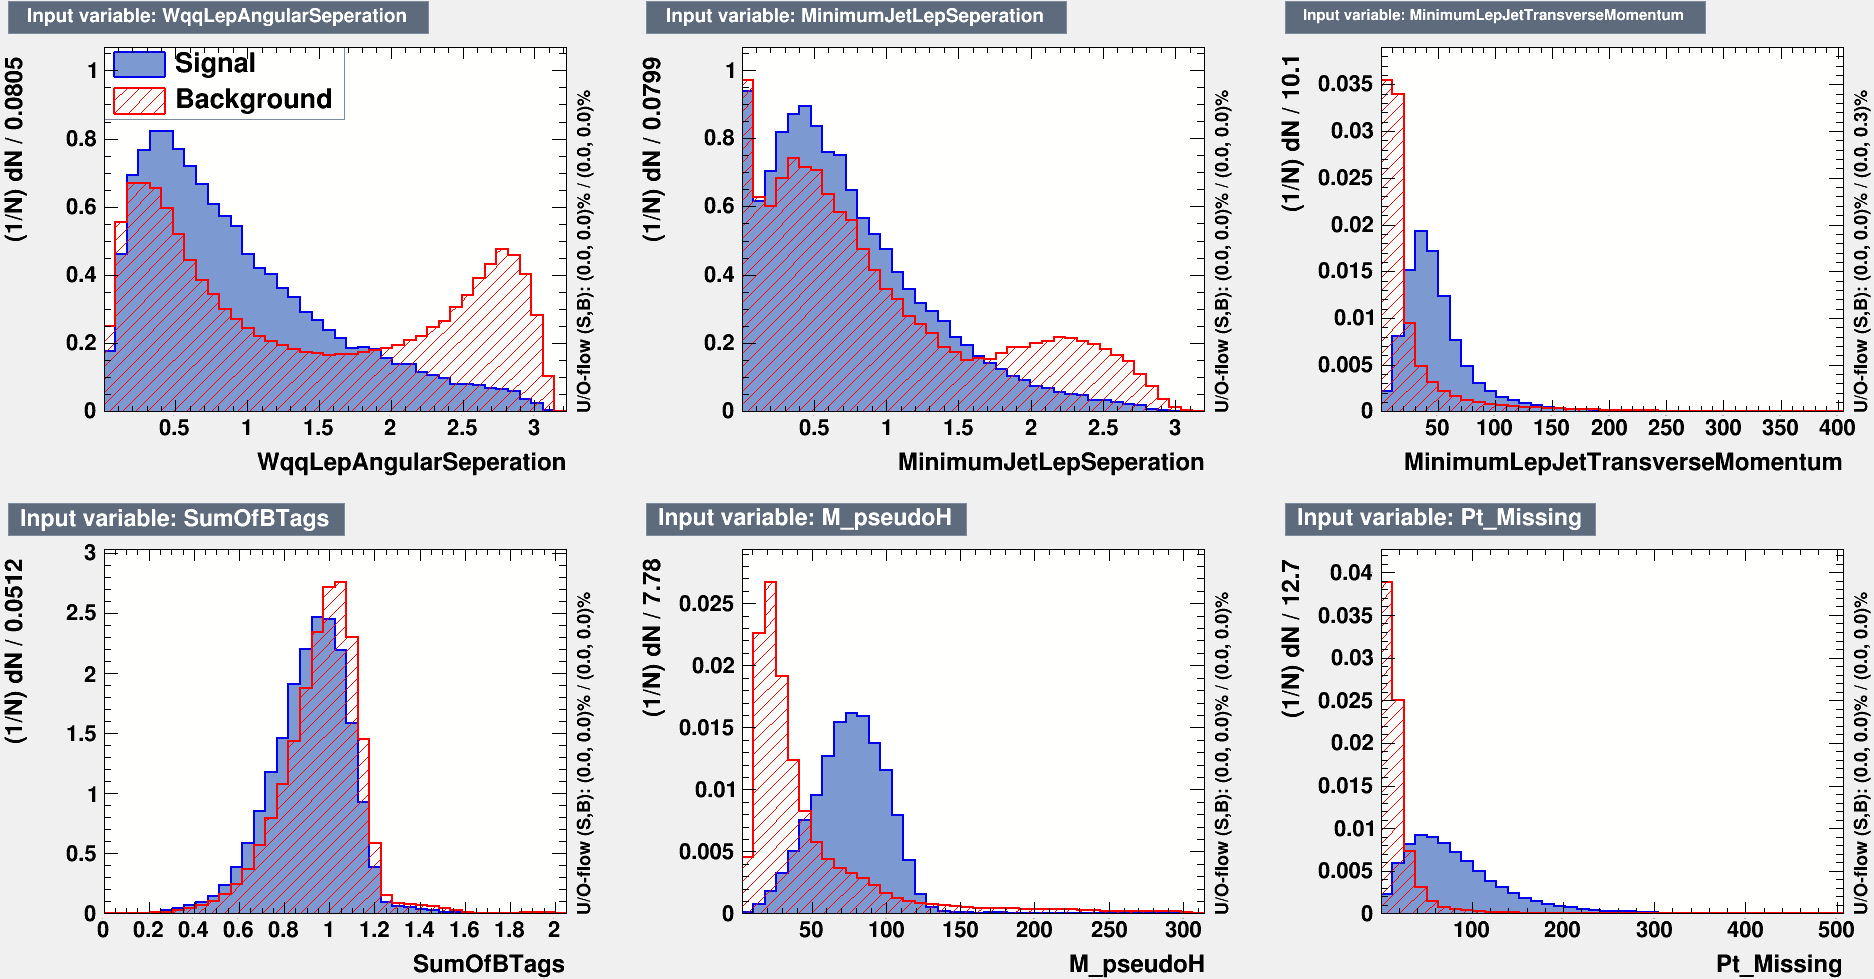
\includegraphics[width=1\linewidth]{figures/variables1}
    \caption{}
    \label{1} 
  \end{subfigure}
  \begin{subfigure}[b]{1.0\textwidth}
    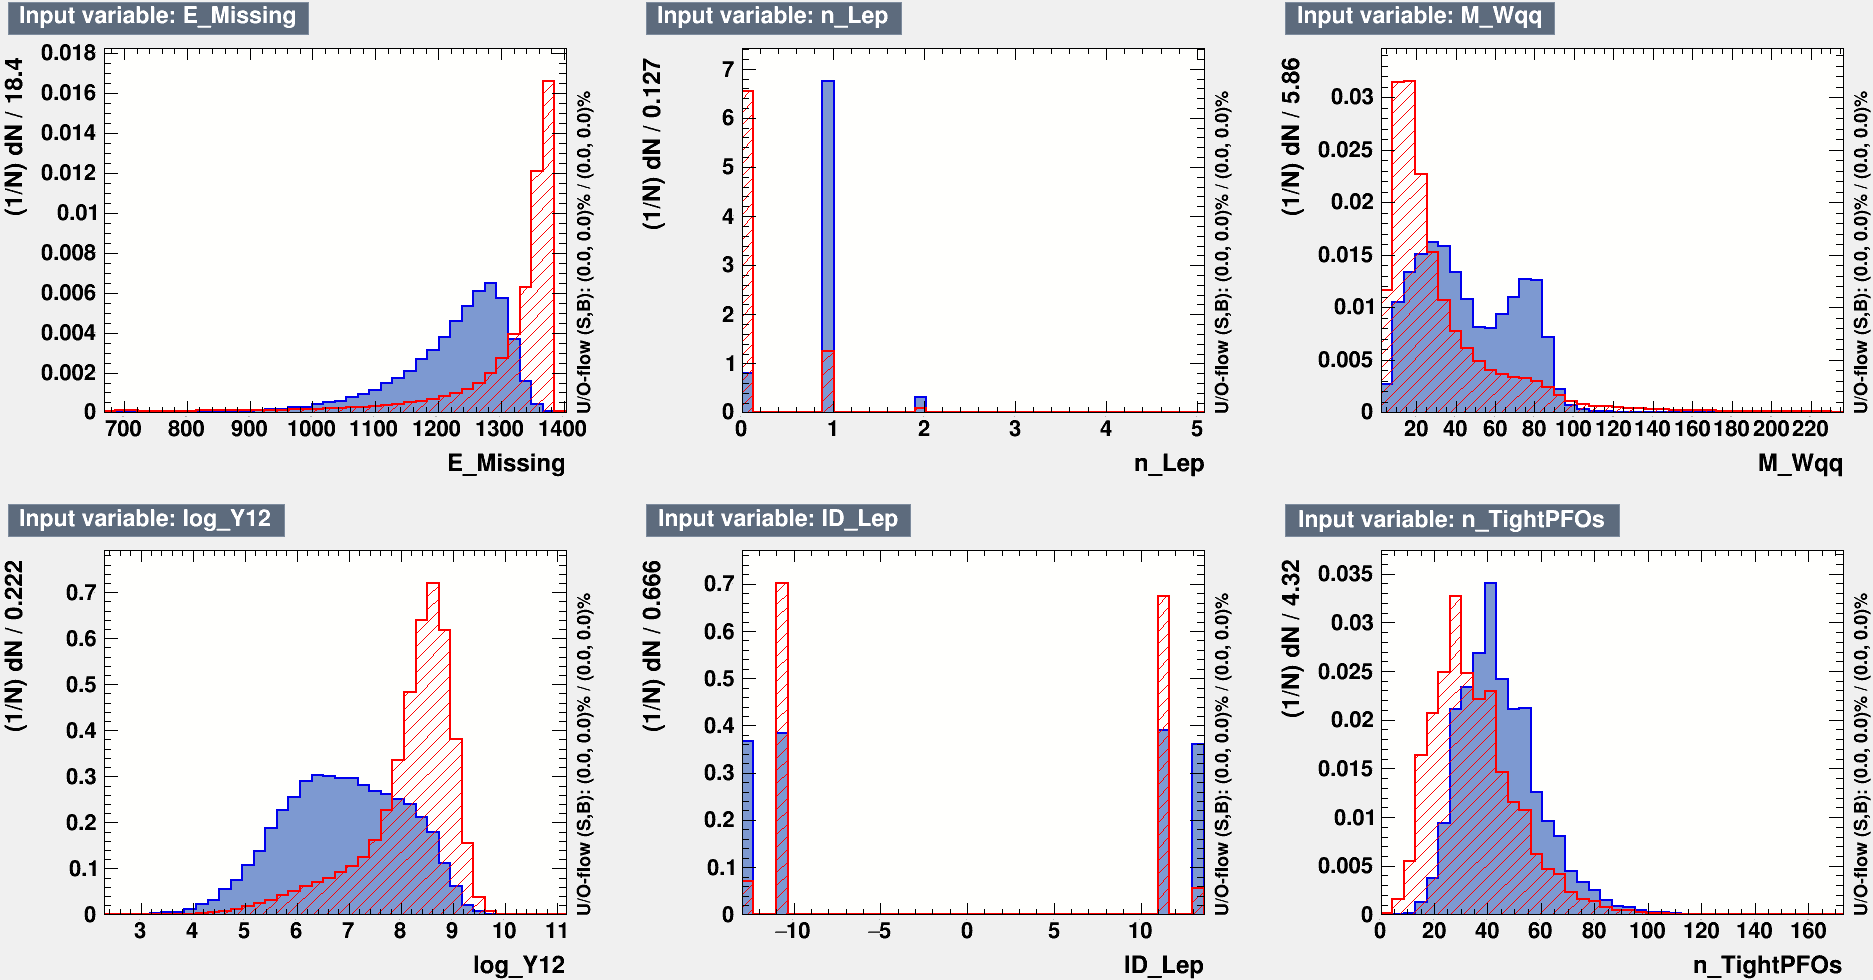
\includegraphics[width=1\linewidth]{figures/variables2}
    \caption{}
    \label{2}
  \end{subfigure}
    \caption{Input variable distributions for training of BDT}
\end{figure}

\begin{figure}[h]
  \centering
  \captionsetup[subfigure]{labelformat=empty}
  \begin{subfigure}[b]{1.0\textwidth}
    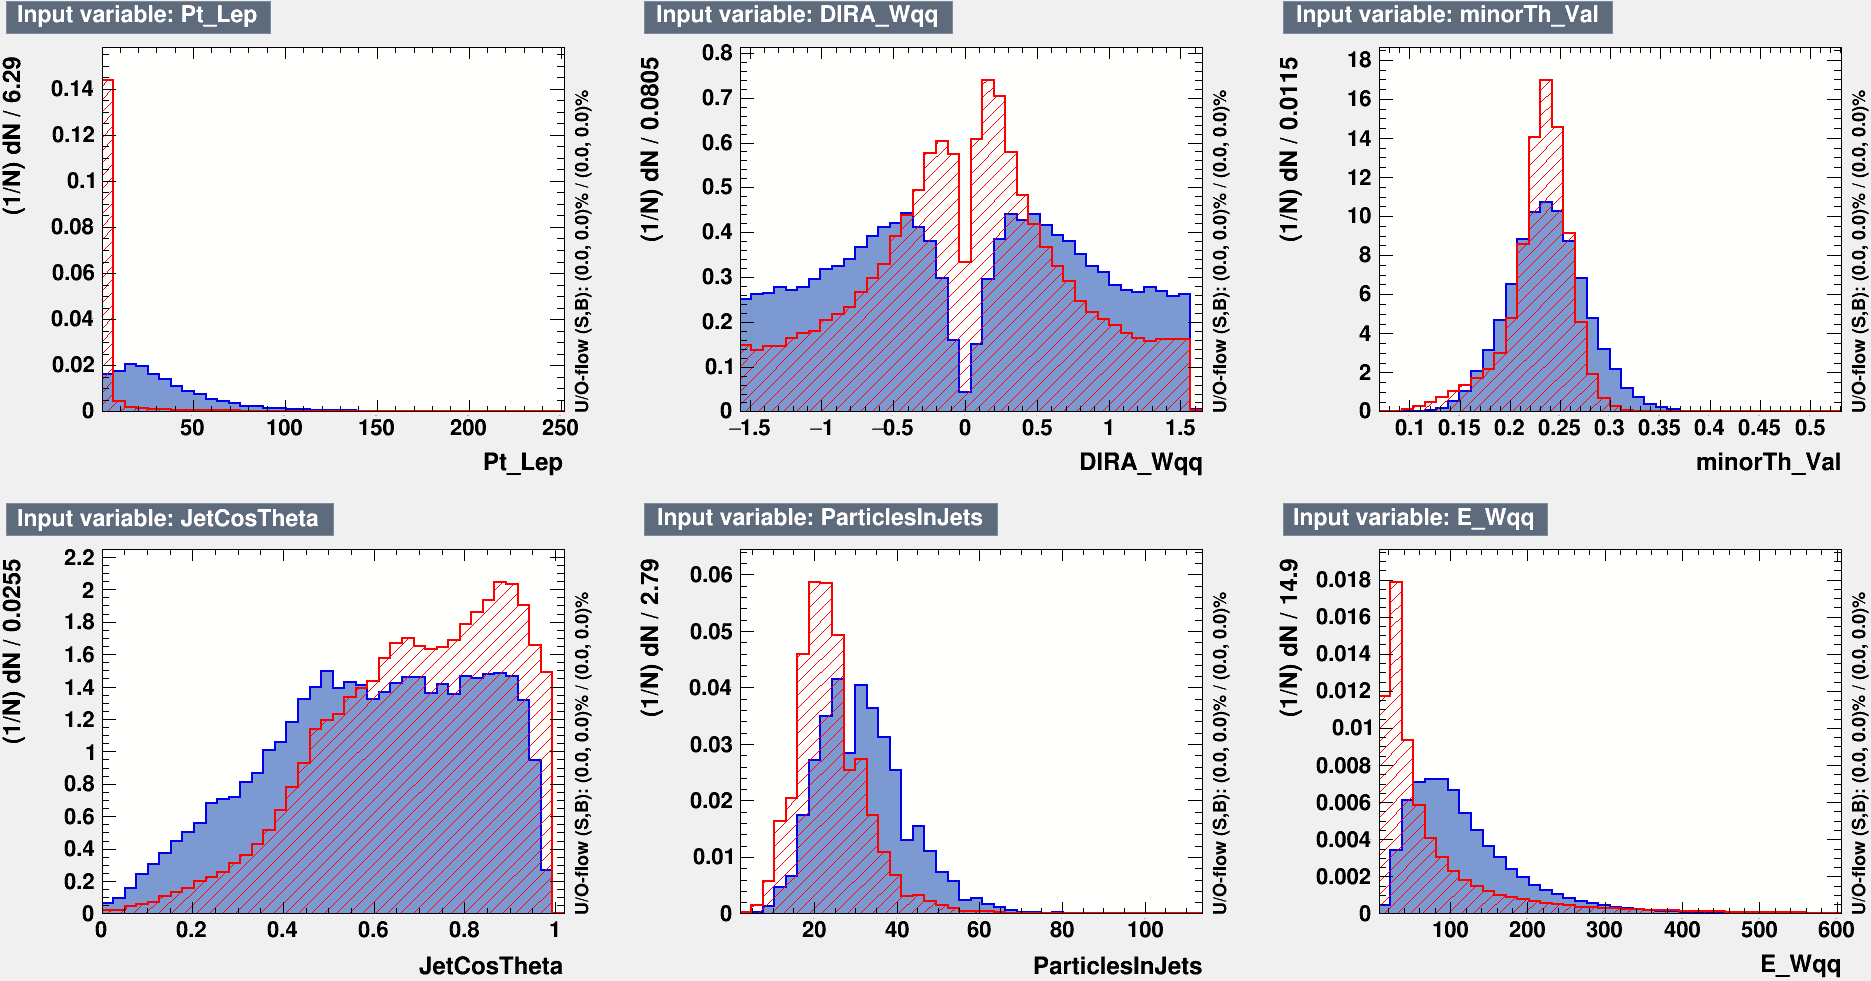
\includegraphics[width=1\linewidth]{figures/variables3}
    \caption{}
    \label{3}
  \end{subfigure}
  \begin{subfigure}[b]{1.0\textwidth}
    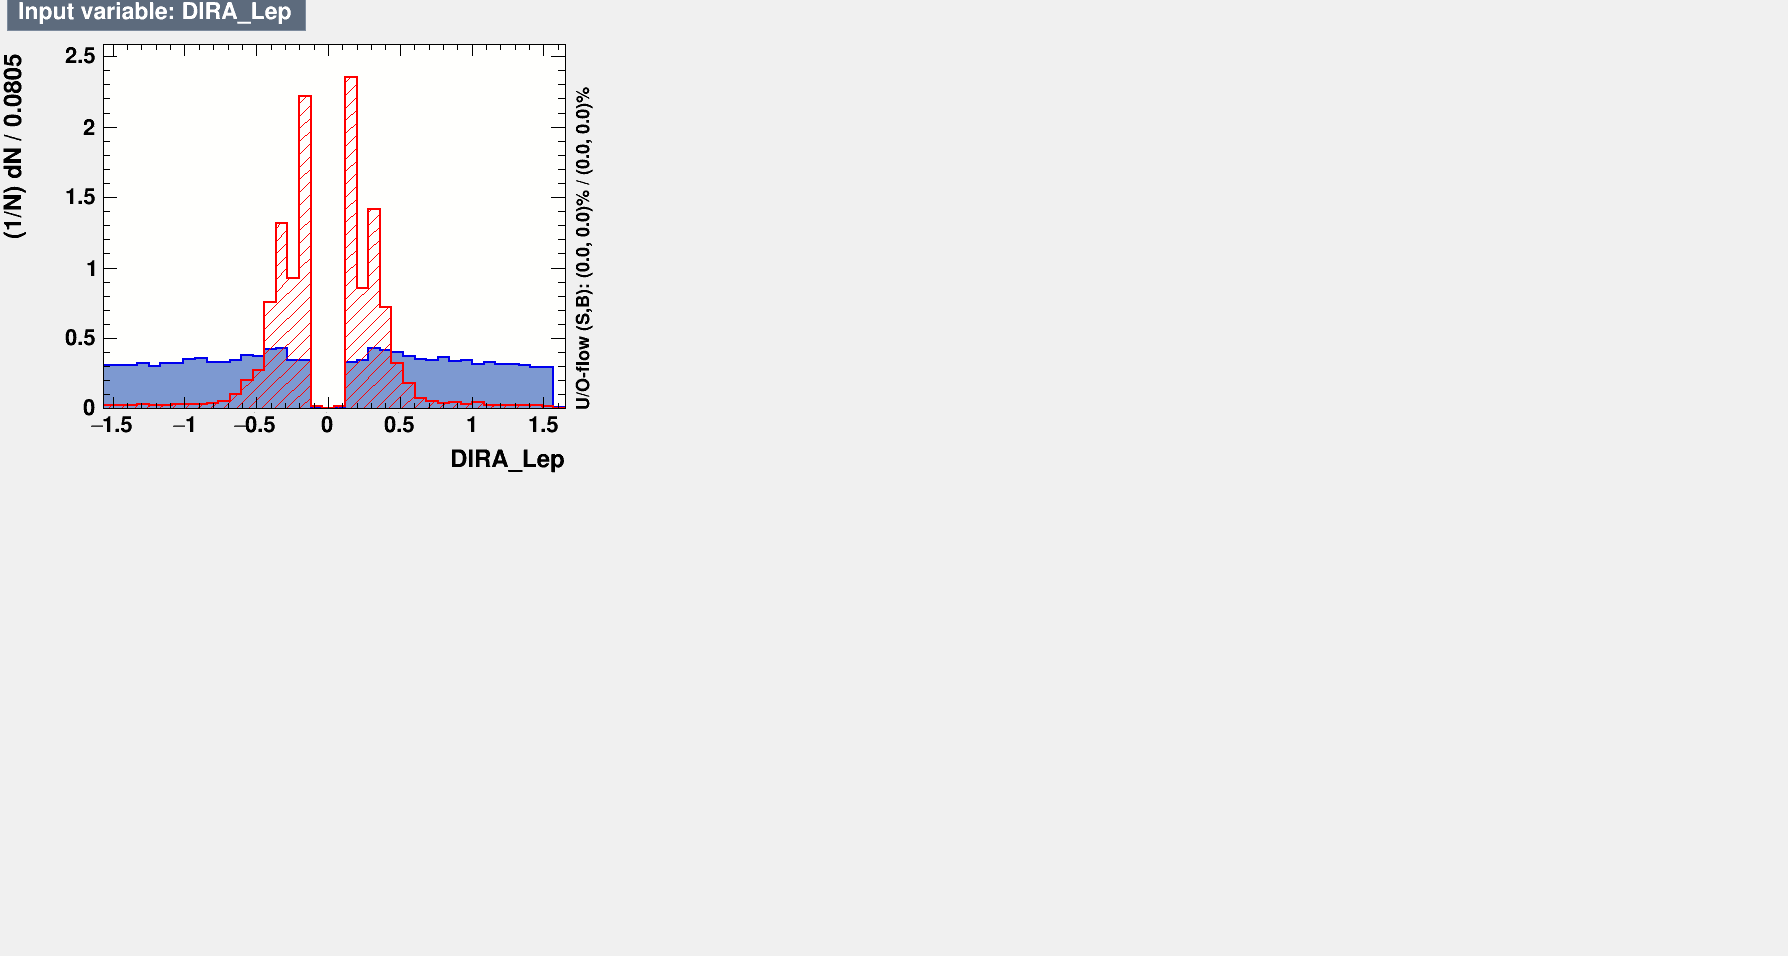
\includegraphics[width=1\linewidth]{figures/variables4}
    \caption{}
    \label{4}
  \end{subfigure}
      \caption{Input variable distributions for training of BDT}
\end{figure}

\clearpage

%\begin{figure}[h]
%  \centering
%  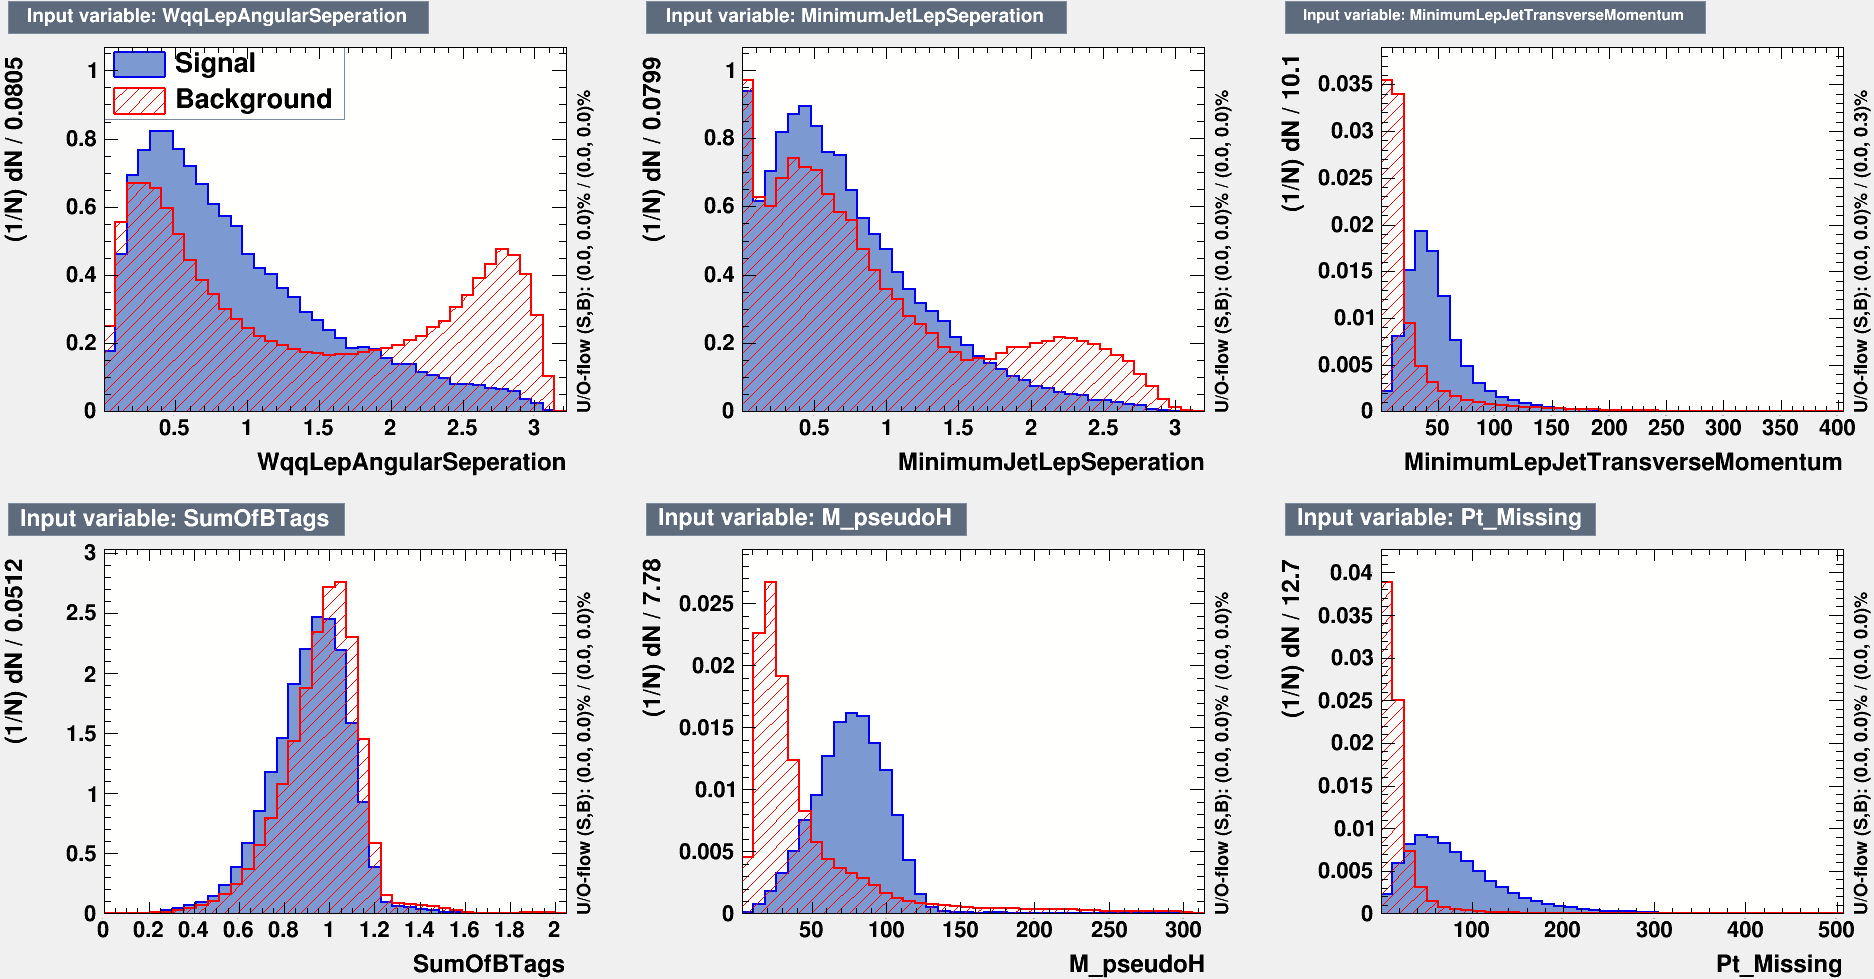
\includegraphics[width=1.0\textwidth,height=12cm,keepaspectratio]{figures/variables1}
%  \label{variables1}
%\end{figure}

%\clearpage
